\documentclass{tufte-book}
\usepackage[utf8]{inputenc}
\usepackage{tikz}
\usepackage[siunitx, american]{circuitikz}
\usepackage{amsmath,amsthm,amssymb}
\usepackage{eso-pic}
\usepackage[dvipsnames]{xcolor}
\usepackage{scalerel}
\usepackage{graphicx}
\graphicspath{{../images/}}

% emoji
\def\light{\scalerel*{
\includegraphics{1F4A1.pdf}}{X\rule[-.3ex]{10pt}{20pt}}}
\def\hat{\scalerel*{
\includegraphics{1F3A9.pdf}}{X\rule[-.3ex]{10pt}{20pt}}}
\def\book{\scalerel*{
\includegraphics{1F4D5.pdf}}{X\rule[-.3ex]{10pt}{20pt}}}
\def\battery{\scalerel*{
\includegraphics{1F50B.pdf}}{X\rule[-.3ex]{10pt}{20pt}}}
\def\bolt{\scalerel*{
\includegraphics{26A1.pdf}}{X\rule[-.3ex]{10pt}{20pt}}}

% cover photo
\newcommand\BackgroundPic{%
\put(-225,-355){%
\parbox[b][\paperheight]{\paperwidth}{%
\vfill
\centering
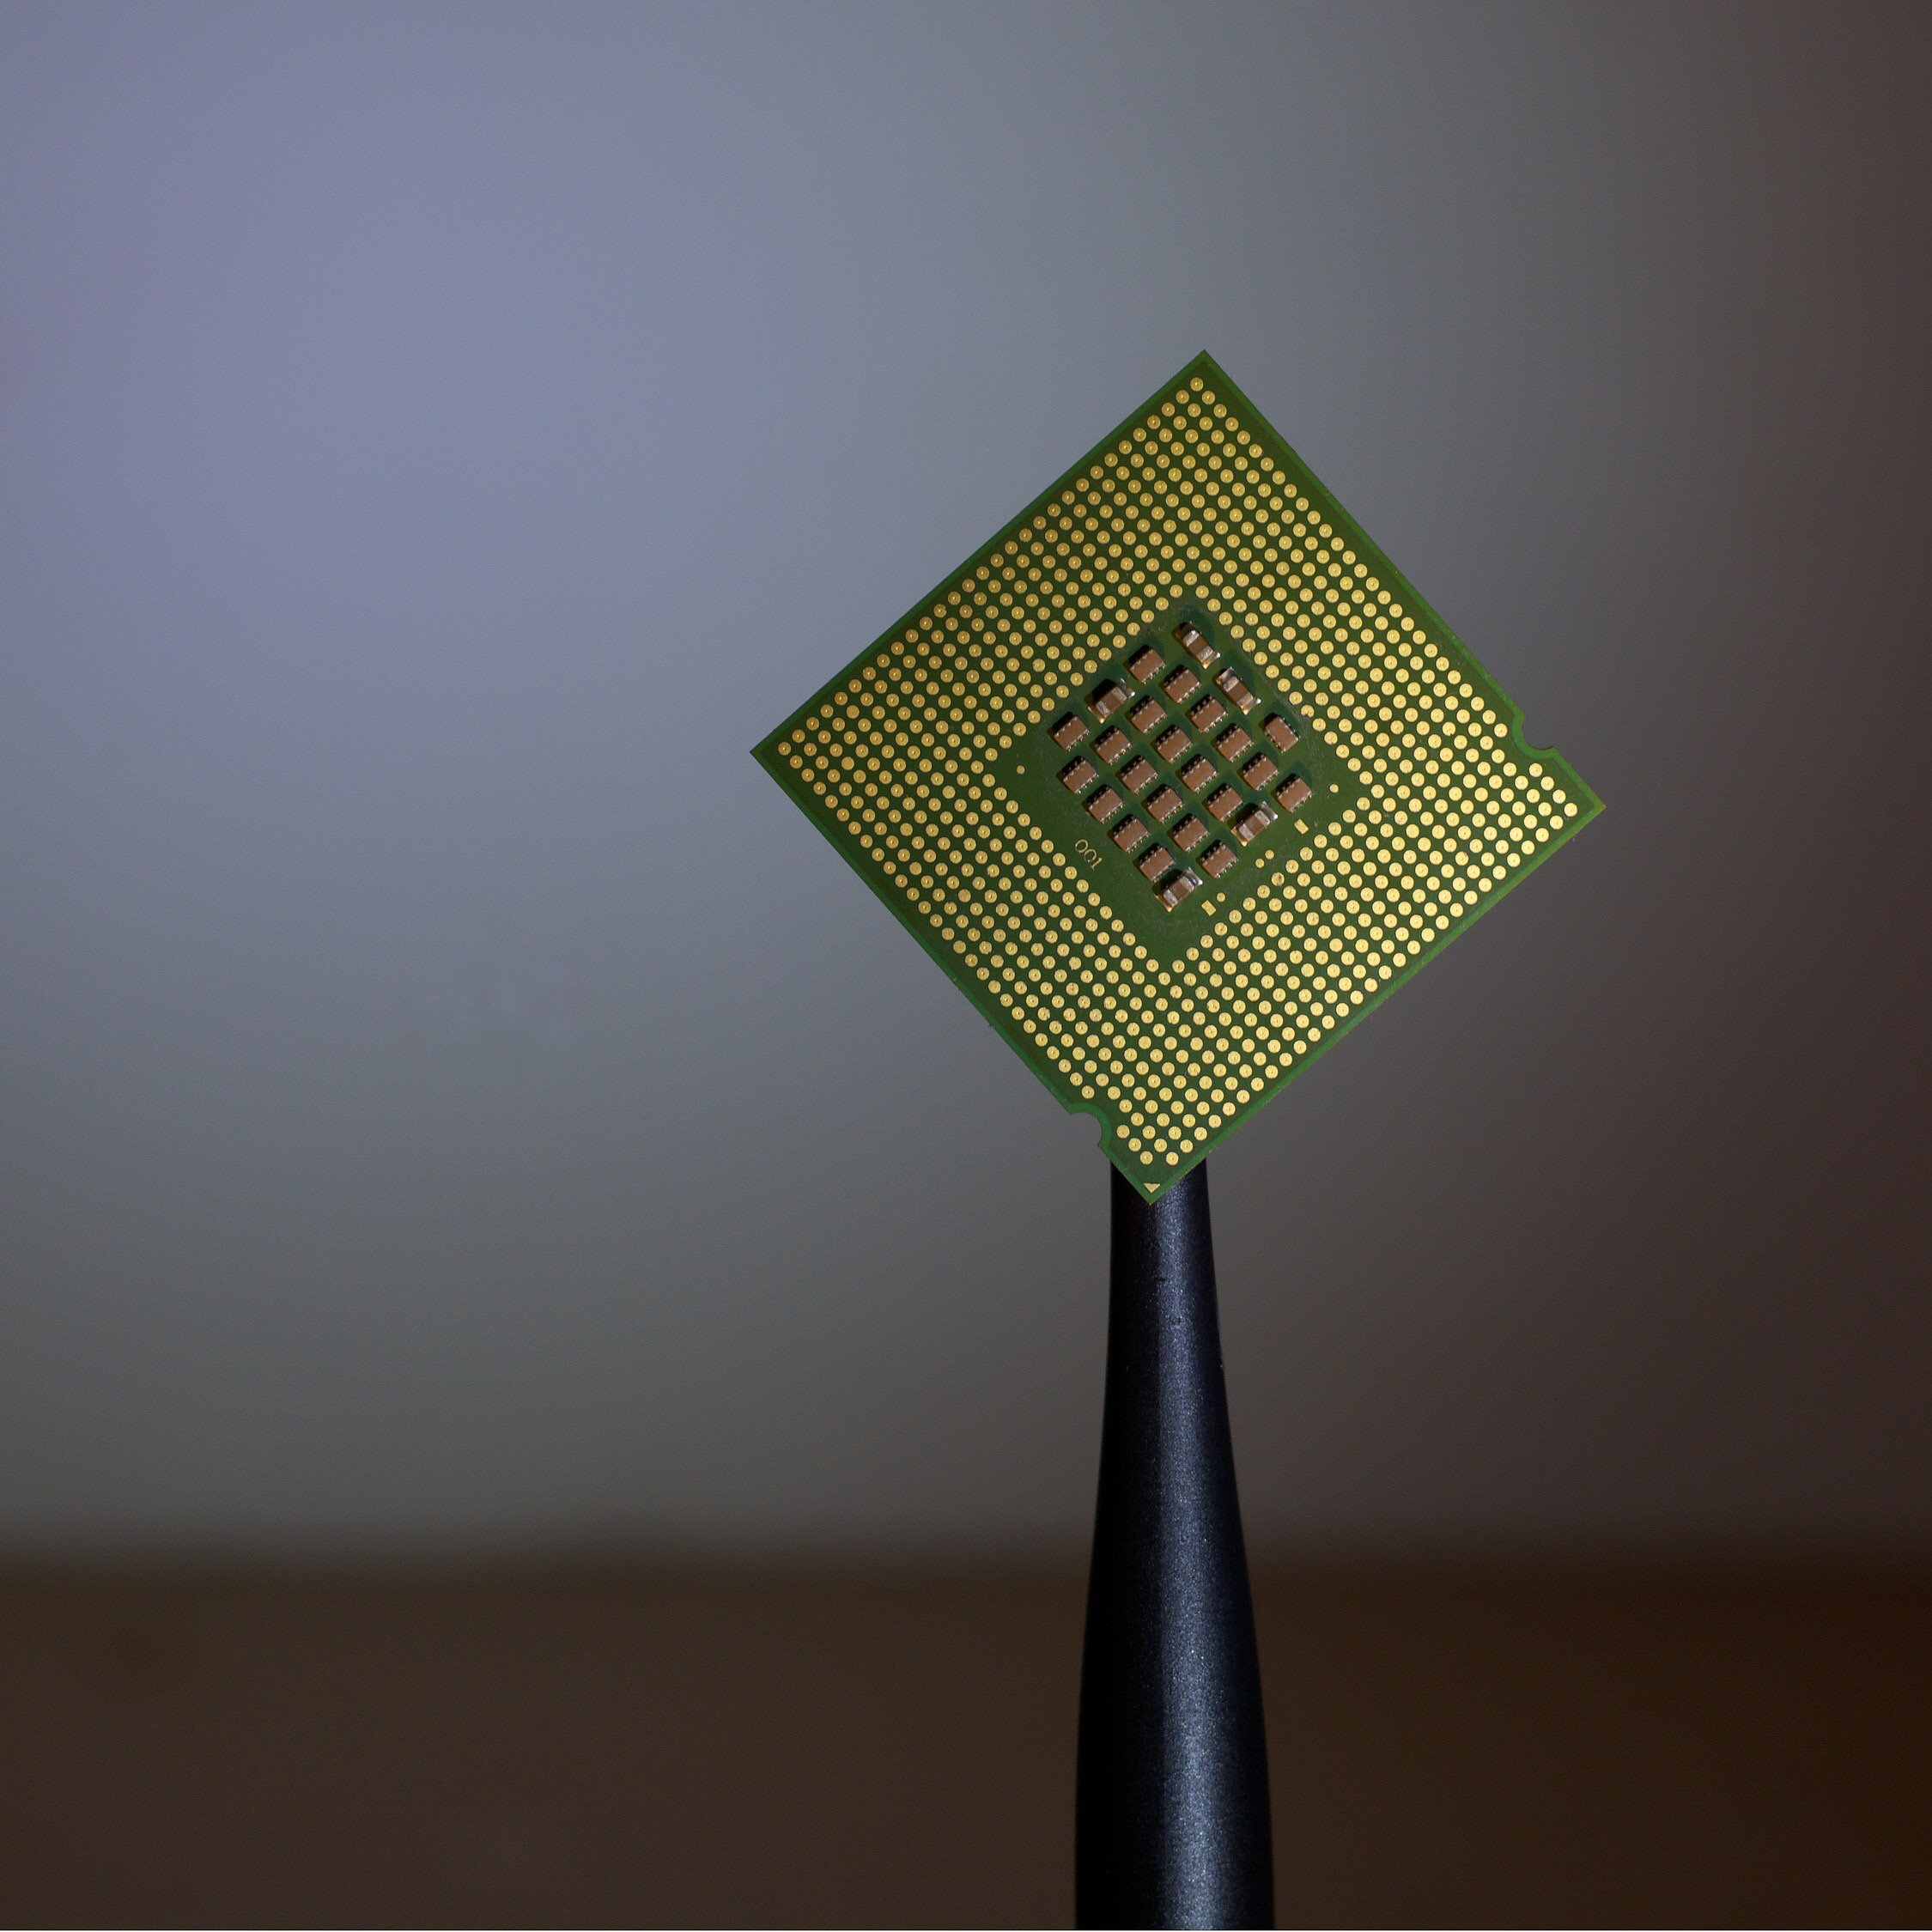
\includegraphics[height=1.45\paperheight,%
keepaspectratio]{circuitscover}%
\vfill
}}}

% circuits
\ctikzset{bipoles/resistor/height=0.15}
\ctikzset{bipoles/resistor/width=0.4}
\ctikzset{bipoles/americaninductor/height=0.15}
\ctikzset{bipoles/americaninductor/width=0.4}
\ctikzset{bipoles/twoport/height=0.5}
\ctikzset{bipoles/twoport/width=0.5}

% title
\setlength{\parindent}{0pt}
\colorlet{darkgray}{white!15!black}
\title[Electronic Circuits]{%
  \setlength{\parindent}{0pt}%
Electronic \par Circuits}
\author{Richard Robinson}
\begin{document}
\AddToShipoutPicture*{\BackgroundPic}
\frontmatter
\maketitle
\setlength{\parindent}{0pt}
\mainmatter

%%%%%%%%%%%%%%%%%%%%%%%%%%%%%%%%%%%%%%%%%%%%%%%%%%%%%%%%%%%%%%%%%%%%%%
% MAIN DOCUMENT
%%%%%%%%%%%%%%%%%%%%%%%%%%%%%%%%%%%%%%%%%%%%%%%%%%%%%%%%%%%%%%%%%%%%%%

\chapter{Analysis Methods \;\protect\book{}}

\section{Definitions}

\textsc{The passive sign convention} states that an impedance's voltage and current are positive if its reference current is in the direction of the voltage drop; that is, from positive to negative. For resistive circuits, \textbf{power} is defined as
%
\begin{marginfigure}
  \begin{center}
    \begin{circuitikz}[line width=0.7pt, line join=round]
      \draw (0,0)
      to [V,l=$v_s$,i>=$ $,*-*] (2.5,0);
    \end{circuitikz} \phantom{mmm}
  \end{center}
  \caption{An independent voltage source.}
\end{marginfigure}
%
\begin{marginfigure}
  \begin{center}
    \begin{circuitikz}[line width=0.7pt, line join=round]
      \draw (0,0)
      to [current source,l=$i_s$,*-*] (2.5,0);
    \end{circuitikz}  \phantom{mmm}
  \end{center}
  \caption{An independent current source.}
\end{marginfigure}
%
\begin{equation}
  p = dw/dt = vi
\end{equation}
For dependent sources the voltage or current values $s$ are denoted by diamonds and given by
\begin{equation}
  x_s = \alpha y_x
\end{equation}
where $y_x$ is the controlling sources. Voltage and current are related through \textbf{Ohm's law},
\begin{equation}
  \mathbf V = Z \mathbf I \quad\text{for}\quad Z = \{R, j \omega L, -j/\omega C \}
\end{equation}
where $Z$ is the \textbf{impedance.}

\bigskip
\textbf{Kirchoff's Laws} for circuit analysis state that the sum of all currents at a node equals zero (KCL) as does the sum of all voltages across a loop (KVL).

\section{Simple Analysis Methods}

The voltage across branches in parallel are equal, as are currents across branches in series. Otherwise, \textbf{voltage} and \textbf{current division} must be used, in which:
%
\begin{marginfigure}
  \begin{center}
    \begin{circuitikz}[line width=0.7pt, line join=round]
      \draw (0,1.5)
      to [open, *-*] (0,0);
      \draw (0,1.5)
      to [open, v^=$v$] (0,0);
      \draw (0,1.5)
      to [R] (1.5,1.5)
      to [R] (3,1.5)
      to [R, l_=$R_j$] (3,0)
      to [R] (1.5,0)
      to [R] (0,0);
      \draw (3,1.5) to [open, v^=$v_j$] (3,0);
    \end{circuitikz}
  \end{center}
  \caption{A circuit for voltage division.}
\end{marginfigure}
%
\begin{marginfigure}
  \begin{center}
    \begin{circuitikz}[line width=0.7pt, line join=round]
      \draw (0,0) to [open, *-*] (0,1.5);
      \draw (0,1.5)
      to [short, i=$i$, *-*] (1,1.5)
      to [R, *-*] (1,0)
      to [short, *-*] (0,0);
      \draw (1,1.5) -- (2,1.5)
      to [R,l_=$R_j$, *-*] (2,0) -- (1,0);
      \draw (2,1.5) -- (3,1.5)
      to [R,*-*] (3,0) -- (2,0);
      \draw (3,1.5) to [open, v^=$v$] (3,0);
    \end{circuitikz}
  \end{center}
  \caption{A circuit for current division.}
\end{marginfigure}
%
\begin{equation}
  v_x = \frac{Z_x}{Z_{eq}} v_s \quad\text{and}\quad i_x = \frac{Z_t}{Z_x + Z_t} i_s
\end{equation}
Furthermore, the \textbf{$\Delta$-to-Y transformation} transforms an interconnection of 3 impedances between the two types in Figures 5 \& 6, converted via:
\begin{equation}
  Z_i = \frac{Z'_{jk}}{\Sigma Z'} \quad\text{and}\quad Z_i' = \frac{P_{jk}}{Z_i}
\end{equation}
where $P_{jk} = Z_iZ_j + Z_iZ_k + Z_jZ_k$.

\section{Nodal Analysis}
The method of \textbf{nodal analysis} is most commonly used when no node in the circuit connects more than three branches. It is done procedurally as follows:
\begin{enumerate}
  \item Select the node with the most branches as the reference node, typically the bottom--most one.
  \item Define the node voltages $v_i$, which are the voltage rises across a branch or branches from the reference node to another node $i$.
  \item For each nonreference node, generate a KCL equation: \begin{equation}
    v_a : \sum i_a = \sum \frac{v_a-v_s}{Z_i} = 0
  \end{equation}
  and solve for $v_i$.
  \item If a voltage source is between two nodes, a supernode exists in which the nodes are related by $v_i = v_j + \alpha y_x$.
\end{enumerate}

\section{Mesh Analysis}
Consequently, the \textbf{mesh analysis} method is most commonly used when there is a node connecting more than three branches. It is also done procedurally as follows:
\begin{enumerate}
  \item Assign mesh current directions around each loop, typically clockwise.
  \item For all nodes, develop individual KCL equations.
  \item For each mesh, generate a KVL equation: \begin{equation}
    v_a : \sum v_a = \sum (i_a - i_i) Z_i = 0
  \end{equation}
  where $i_i$ is any other mesh current passing through $Z$.
  \item Solve for the branch currents, letting $i_a = i_\alpha$; if a branch is shared, $i_\alpha = i_a - i_b$. Then solve the system of equations.
\end{enumerate}

\section{Source Transformations}
The \textbf{source transformation} technique states a voltage $v_s = i_sZ$ source in series with an impedance $Z$ (Thévenin equivalent) is equivalent to a current source $i_s$ in parallel with the same impedance (Norton equivalent). As well, an impedance in parallel with $v_s$ or in series with $i_s$ has no effect and may be directly removed.

\bigskip
Any linear circuit $N$ which is converted to a Thévenin equivalent between a pair of terminals is known as a \textbf{Thévenin} circuit, shown below.

\section{Thévenin's Theorem}

This circuit is especially useful for calculating the current and voltage of the terminals of the load $Z_L$. To calculate $V_T$, replace $Z_L$ with an open circuit and find the voltage drop across the open circuit, typically via voltage division. There are several methods to find $Z_T$:

\bigskip
\textbf{Method 1 (All Sources)}: The current $i_{sc}$ is found by replacing $Z_L$ with a short circuit and calculating the resulting current. Therefore, the Thévenin impedance is
\begin{equation}
 Z_T = V_T/i_{sc}
\end{equation}
\textbf{Method 2 (Independent Sources)}:  Deactivate all independent sources, then calculate the equivalent impedance $Z_{eq}=Z_T$ for the network.

\bigskip
\textbf{Method 3 (Dependent Sources)}: Deactivate all independent sources, then apply a test source between the terminals. The Thévenin impedance is then \begin{equation}
 Z_T = V_{sc}/i_{sc}
\end{equation}

\section{Superposition}

The principle of \textbf{superposition} states suppressing all but one source sequentially and summing the values is equivalent to the original circuit. To suppress a voltage course is to replace it with a short circuit, and an open circuit for a current source.

\bigskip
Specifically, for a circuit with $n$ independent sources, a maximum of $n$ superposition circuits may be created with one source activated per circuit. Therefore, the total current or voltage $x = \sum x_i$.


\end{document}
